\documentclass[]{beamer}

\usepackage[utf8]{inputenc}
\usepackage{lmodern}

\usepackage{listings}

\usepackage{graphicx}
\usepackage{xcolor}
\usepackage{tikz}
\usetikzlibrary{arrows, snakes, backgrounds}
\usepackage{wrapfig}

\title{Umgehen von USB-Deskriptor basierten USB-Richtlinien}
\subtitle{am Beispiel einer Virtual Desktop Infrastrukture Umgebung}
\date{\today}
\author{Dominik Gunther Florian Schlecht}
\institute[THI]{Technische Hochschule Ingolstadt}


\useoutertheme{infolines}
\useinnertheme{circles}

\definecolor{THIblue}{rgb}{0.0078,0.1176,0.4705}

%\setbeamercolor{alerted text}{fg=blue}
\setbeamercolor{background canvas}{bg=white}	%Hintergrund
%\setbeamercolor{block body alerted}{bg=normal text.bg!90!black}
%\setbeamercolor{block body alerted}{bg=blue text.bg=blue}
%\setbeamercolor{block body}{bg=normal fg=green}
%\setbeamercolor{block body example}{bg=normal fg=green}
%\setbeamercolor{block title alerted}{use={normal text,alerted text},fg=alerted text.fg!75!normal text.fg,bg=normal text.bg!75!black}
%\setbeamercolor{block title}{bg=green}
%\setbeamercolor{block title example}{use={normal text,example text},fg=example text.fg!75!normal text.fg,bg=normal text.bg!75!black}
%\setbeamercolor{fine separation line}{}
\setbeamercolor{frametitle}{bg=white,fg=THIblue} %Folientitel
%\setbeamercolor{item projected}{fg=green}
\setbeamercolor{normal text}{fg=black}	%Normaler Text
%\setbeamercolor{palette sidebar primary}{use=normal text,fg=normal text.fg}
%\setbeamercolor{palette sidebar quaternary}{use=structure,fg=structure.fg}
%\setbeamercolor{palette sidebar secondary}{use=structure,fg=structure.fg}
%\setbeamercolor{palette sidebar tertiary}{use=normal text,fg=normal text.fg}
%\setbeamercolor{section in sidebar}{fg=brown}
%\setbeamercolor{section in sidebar shaded}{fg=grey}
%\setbeamercolor{separation line}{}
%\setbeamercolor{sidebar}{bg=red}
%\setbeamercolor{sidebar}{parent=palette primary}
\setbeamercolor{structure}{bg=lightgray, fg=THIblue}
%\setbeamercolor{subsection in sidebar}{fg=green}
%\setbeamercolor{subsection in sidebar shaded}{fg=green}
\setbeamercolor{title}{fg=THIblue}
%\setbeamercolor{titlelike}{fg=green}

\AtBeginSection[]
{
  \begin{frame}[Inhaltsverzeichnis]
    \frametitle{Table of Contents}
    \tableofcontents[currentsection]
  \end{frame}
}

\begin{document}
	\frame{\maketitle}
	\frame{\tableofcontents}
	
	\section{Problem- und Fragestellung}
	\begin{frame}{\secname}
		Einige Mitarbeiter im Backoffice brauchen eine Möglichkeit, CDs zu lesen. 
		\pause		
		Da diese an Thin-Clients arbeiten, ist dies derzeit nicht gegeben.
		\pause
		\begin{figure}[htbp]
			\centering
			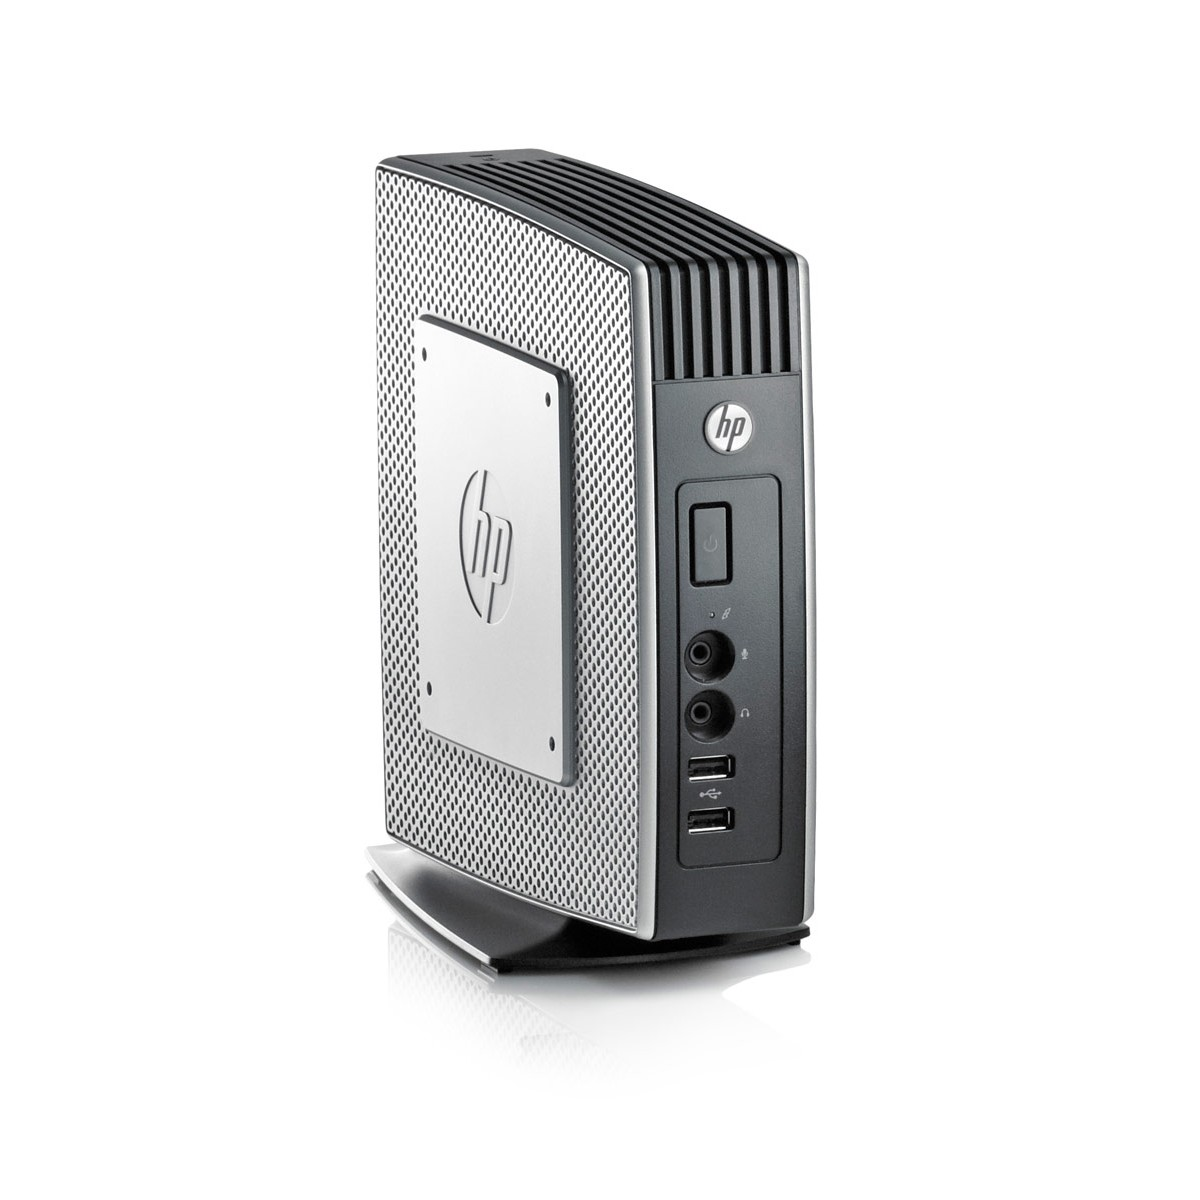
\includegraphics[width=0.375\textwidth]{bilder/thinclient.jpg}
			\caption{HP Thin-Client}
			\label{fig:Thin-Client}
		\end{figure}
	\end{frame}
	
	\begin{frame}{\secname}
		Idee:
		\begin{itemize}
			\item Für wenige Mitarbeiter genau 2 Arten von CD-USB-Laufwerken durchstellen.
			\item Dies soll anhand der Richtlinien am Hypervisor reguliert werden.
		\end{itemize}
		\pause
		$ $\newline
		Kritische Frage:
		\begin{itemize}
			\item Kann anhand der Richtline sichergestellt werden, dass keine anderen Geräte durchgestellt werden?
		\end{itemize}
	\end{frame}
	
	\section{USB-Deskriptoren}
	\begin{frame}{\secname}
		Jedes USB-Gerät übergibt beim Einstecken bestimmte Deskriptorfelder:
		\begin{wrapfigure}{l}{0pt}
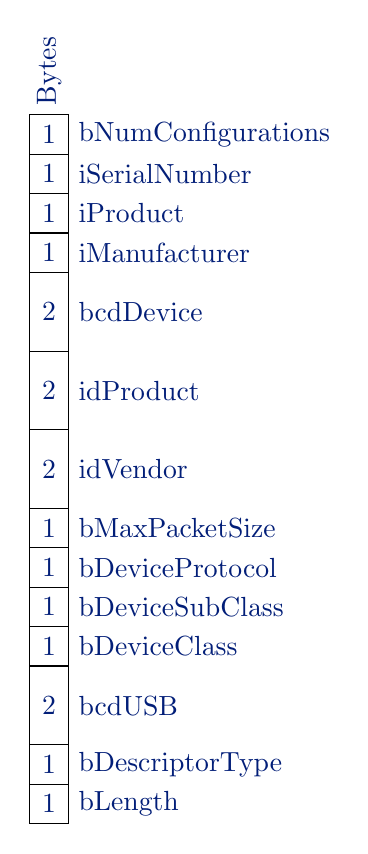
\begin{tikzpicture}[scale=1, text=THIblue]
	\draw (0,0) rectangle (0.5,0.5);
	\draw (0.25, 0.25) node {1};
	\draw (0.5, 0.25) node[right]{bLength};
	
	\draw (0,0.5) rectangle (0.5,0.5);
	\draw (0.25, 0.75) node {1};
	\draw (0.5, 0.75) node[right]{bDescriptorType};
	
	\draw (0,1) rectangle (0.5,1);
	\draw (0.25,1.5) node {2};
	\draw (0.5,1.5) node[right]{bcdUSB};
	
	\draw (0,2) rectangle (0.5,0.5);
	\draw (0.25,2.25) node {1};
	\draw (0.5,2.25) node[right]{bDeviceClass};

	\draw (0,2.5) rectangle (0.5,0.5);
	\draw (0.25,2.75) node {1};
	\draw (0.5,2.75) node[right]{bDeviceSubClass};

	\draw (0,3) rectangle (0.5,0.5);
	\draw (0.25,3.25) node {1};
	\draw (0.5,3.25) node[right]{bDeviceProtocol};

	\draw (0,3.5) rectangle (0.5,0.5);
	\draw (0.25,3.75) node {1};
	\draw (0.5,3.75) node[right]{bMaxPacketSize};
	
	\draw (0,4) rectangle (0.5,1);
	\draw (0.25,4.5) node {2};
	\draw (0.5,4.5) node[right]{idVendor};
	
	\draw (0,5) rectangle (0.5,1);
	\draw (0.25,5.5) node {2};
	\draw (0.5,5.5) node[right]{idProduct};
	
	\draw (0,6) rectangle (0.5,1);
	\draw (0.25,6.5) node {2};
	\draw (0.5,6.5) node[right]{bcdDevice};
	
	\draw (0,7) rectangle (0.5,0.5);
	\draw (0.25,7.25) node {1};
	\draw (0.5,7.25) node[right]{iManufacturer};
	
	\draw (0,7.5) rectangle (0.5,0.5);
	\draw (0.25,7.75) node {1};
	\draw (0.5,7.75) node[right]{iProduct};
	
	\draw (0,8) rectangle (0.5,0.5);
	\draw (0.25,8.25) node {1};
	\draw (0.5,8.25) node[right]{iSerialNumber};
	
	
	\draw (0,8.5) rectangle (0.5,0.5);
	\draw (0.25,8.75) node {1};
	\draw (0.5,8.75) node[right]{bNumConfigurations};
	
	\draw (0,9) rectangle (0.5,0.5);
	
	\draw (0.25, 9) node[rotate=90, right] {Bytes};
\end{tikzpicture}
\label{fig:usbDeskriptoren}
\end{wrapfigure}
	\end{frame}
	
	\section{USB-Richtlinien am Hypervisor}
	\begin{frame}{\secname}
		Aufbau:
		\begin{itemize}
			\item Verbiete alle USB-Geräte \textit{ODER}
			\item Benutzer ist Alice \textit{DANN}
			\begin{itemize}
				\item Verbiete alle USB-Geräte \textit{ODER}
				\begin{itemize}
					\item Das Gerät besitzt \textit{idProduct=0x01} \textit{UND}
					\item Das Gerät besitzt \textit{idVendor=0x02} \textit{DANN}
					\item Stelle das Gerät zur Virtuellen Machine durch		
				\end{itemize}
			\end{itemize}						
			
		\end{itemize}
	\end{frame}

	\section{Teensy}
	\begin{frame}{\secname}
		\begin{figure}[htbp]
			\centering
			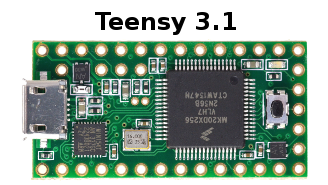
\includegraphics[width=0.5\textwidth]{bilder/teensy31.png}
			\caption{Teensy 3.1}
			\label{fig:Teensy}
		\end{figure}
	\end{frame}
	\section{Demonstration}

	\begin{frame}{\secname}
		Demo!
	\end{frame}
	
\end{document}